% Created 2021-09-11 Sat 09:36
% Intended LaTeX compiler: xelatex
\documentclass[letterpaper]{article}
\usepackage{graphicx}
\usepackage{grffile}
\usepackage{longtable}
\usepackage{wrapfig}
\usepackage{rotating}
\usepackage[normalem]{ulem}
\usepackage{amsmath}
\usepackage{textcomp}
\usepackage{amssymb}
\usepackage{capt-of}
\usepackage{hyperref}
\usepackage[margin=1in]{geometry}
\usepackage{fontspec}
\usepackage{indentfirst}
\setmainfont[ItalicFont = LiberationSans-Italic, BoldFont = LiberationSans-Bold, BoldItalicFont = LiberationSans-BoldItalic]{LiberationSans}
\newfontfamily\NHLight[ItalicFont = LiberationSansNarrow-Italic, BoldFont       = LiberationSansNarrow-Bold, BoldItalicFont = LiberationSansNarrow-BoldItalic]{LiberationSansNarrow}
\newcommand\textrmlf[1]{{\NHLight#1}}
\newcommand\textitlf[1]{{\NHLight\itshape#1}}
\let\textbflf\textrm
\newcommand\textulf[1]{{\NHLight\bfseries#1}}
\newcommand\textuitlf[1]{{\NHLight\bfseries\itshape#1}}
\usepackage{fancyhdr}
\pagestyle{fancy}
\usepackage{titlesec}
\usepackage{titling}
\makeatletter
\lhead{\textbf{\@title}}
\makeatother
\rhead{\textrmlf{Compiled} \today}
\lfoot{\theauthor\ \textbullet \ \textbf{2021-2022}}
\cfoot{}
\rfoot{\textrmlf{Page} \thepage}
\titleformat{\section} {\Large} {\textrmlf{\thesection} {|}} {0.3em} {\textbf}
\titleformat{\subsection} {\large} {\textrmlf{\thesubsection} {|}} {0.2em} {\textbf}
\titleformat{\subsubsection} {\large} {\textrmlf{\thesubsubsection} {|}} {0.1em} {\textbf}
\setlength{\parskip}{0.45em}
\renewcommand\maketitle{}
\author{Houjun Liu}
\date{\today}
\title{Gravitational Potential and Center of Mass}
\hypersetup{
 pdfauthor={Houjun Liu},
 pdftitle={Gravitational Potential and Center of Mass},
 pdfkeywords={},
 pdfsubject={},
 pdfcreator={Emacs 27.2 (Org mode 9.4.4)}, 
 pdflang={English}}
\begin{document}

\maketitle

\section{Escape Velocity and Gravitational Potential Energy}
\label{sec:org21a5741}

\subsection{Newton's Universal Gravitation Law}
\label{sec:org94caedf}
\begin{equation}
\vec{F_g} = - \frac{GM_1M_2}{r^2} \hat{r}
\end{equation}

where, \(\vec{F_g}\) is the force of gravity on \(M_2\); \(M_1\) and \(M_2\) are two point masses; \(G\) the universal gravitation constant; \(r\) the magnitude of the vector \(\vec{r}\) from \(M_1\) to \(M_2\) and \(\hat{r}\) the unit vector in the \(\vec{r}\) direction.

\subsection{Equation for Gravitational Potential Energy}
\label{sec:org7cbd68e}

\subsubsection{Needed Definitions}
\label{sec:org160dba9}
To begin, we need to modify the \hyperref[sec:org94caedf]{Newton's Universal Gravitation Law} to fit the parameters of the scenario. Namely, we need to treat both Earth and our object as point masses, and assign \(M_1\) to be Earth and \(M_2\) to be our object.

Also, it is necessary to define the coordinate system: that our object, \(M_2\), is defined to be to the left/more negative side of the coordinate compared to the location occupied by the Earth, \(M_e=M_1\) (as, per the problem, the "zero" point is set at \(r = \infty\).)

With this assumption, we could therefore claim \(\vec{r}\) to be pointing from the origin to the \emph{negative} side of the axis, rendering it represented by the value \(-1\) for this system.

Hence, with the necessary variable substitutions as highlighted before, we arrive at the following equation:

\begin{equation}
\vec{F_{em}}(r) = \frac{GM_eM_2}{r^2}
\end{equation}

\subsubsection{Deducing Gravitational Potential energy}
\label{sec:org6a5b171}

The general equation for work is as follows:

\begin{equation}
W = F(x) dx
\end{equation}

In this case, as we will be deducing the total gravitational potential energy as per the setup above, we need to be integrating upon \(\vec{F_{em}}(r) dr\). Hence, the integral is therefore:

\begin{equation}
W = \int{\frac{GM_eM_2}{r^2} dr}
\end{equation}

Determining the total gravitation potential energy will therefore involve evaluating the integral:

\begin{eqnarray}
W &=& \int{\frac{GM_eM_2}{r^2} dr} \\
W &=& GM_eM_2 \int{\frac{1}{r^2} dr} \\
W &=& GM_eM_2 \int{r^{-2} dr} \\
W &=& \frac{-GM_eM_2}{r}
\end{eqnarray}

\subsection{Escape Velocity}
\label{sec:org1dca6bc}
To deduct the escape velocity of the Earth, our object \(M_2\) must do enough work such that the work Earth exerts upon it --- \hyperref[sec:org6a5b171]{as deducted above} --- is canceled out.

\subsubsection{Calculation Setup}
\label{sec:org40f3afb}
Hence, to figure the escape velocity, we must deduct the kinetic energy needed to perform the exact work deducted above in the opposite direction. That,

\begin{equation}
-\frac{1}{2}M_2 \vec{V}^2 = \frac{-GM_eM_2}{r}
\end{equation}

Notably, the negative sign before the kinetic energy equation corresponds to the fact that the work is done in an opposite direction as that done by Earth's gravitational potential energy.

Also, as the object to escape Earth's gravitation is starting at the surface of Earth, \(r = R_e\), the radius of the earth.

\subsubsection{Deducing Escape Velocity}
\label{sec:org49d5842}
The final calculations after substitution is therefore simply a matter of isolating \(\vec{V}\), the velocity vector.

\begin{align}
-\frac{1}{2}M_2 \vec{V}^2 &= \frac{-GM_eM_2}{R_e} \\
\vec{V}^2 &= 2\frac{GM_e}{R_e} \\
\vec{V} &= \sqrt{2\frac{GM_e}{R_e}} 
\end{align}

\subsubsection{Calculating Escape Velocity}
\label{sec:org9764edd}
Taking \(G = 6.674 \times 10^{-11} m^3 \frac{m^3}{kg\ s^2}\), \(M_e = 5.97 \times 10^{24} kg\), and \(R_e = 6.371 \times 10^6 km\)\ldots{}

\begin{equation}
|\vec{V}| \approx 1.119 \times 10^4 \frac{m}{s} = 2.503 \times 10^4 \frac{M}{h}
\end{equation}

\section{Center of Mass}
\label{sec:org32cd518}

\subsection{Finding an Expression for the Position of the Center of Mass}
\label{sec:org7e76963}
The net force of a system is described as:

\begin{equation}
\sum^n_{i=1} \vec{F_{net,i}} = (\sum^n_{i=1} m_i) \ddot{\vec{r_{CM}}}
\end{equation}

where, \(\vec{F_{net,i}}\) is the net force on \(m_i\), \(\vec{r_{CM}}\) the position vector of the center of mass \(CM\).

In order to isolate \(\vec{r_{CM}}\), the equation above must be integrated twice w.r.t. time, namely:

\begin{equation}
\int \int \sum^n_{i=1} \vec{F_{net,i}} dt dt = \int \int (\sum^n_{i=1} m_i) \ddot{\vec{r_{CM}}} dt dt
\end{equation}

For this evaluation, we will also set \(\sum^n_{i=1} m_i = M\), define \(\vec{a_i}\) as acceleration of \(m_i\), \(\vec{r_i}\) as position of \(m_i\), and apply Newton's second law:

\begin{align}
\int \int \sum^n_{i=1} \vec{F_{net,i}} dt dt &= \int \int (\sum^n_{i=1} m_i) \ddot{\vec{r_{CM}}} dt dt \\
\int (\sum^n_{i=1} m_i \int \vec{a_i} dt) dt &= \int (M \int \ddot{\vec{r_{CM}}} dt) dt \\
\int (\sum^n_{i=1} m_i \int \frac{d^2\vec{r_i}}{dt^2} dt) dt &= \int (M \int \frac{d^2\vec{r_{CM}}}{dt^2} dt) dt \\
\int (\sum^n_{i=1} m_i \frac{d\vec{r_i}}{dt}) dt &= \int M \frac{d\vec{r_{CM}}}{dt} + C_1 dt \\
\sum^n_{i=1} m_i \int \frac{d\vec{r_i}}{dt} dt &= M \int \frac{d\vec{r_{CM}}}{dt} + C_1 dt \\
\sum^n_{i=1} m_i \vec{r_i} + C_2 &= M \vec{r_{CM}} \\
\frac{1}{M} \sum^n_{i=1} m_i \vec{r_i} + C_2  &= \vec{r_{CM}}
\end{align}

In the case of the first integral application, the constant of integration --- \(C_1\) --- is defined to be zero due to the fact that, were it to be nonzero, the center of mass would be traveling at a faster rate than that of the object. As the object increases in speed, the center of mass would therefore increase in speed as well more than the object: leading it to travel away from the object, which would be absurd.

In the latter case, the constant of integration --- \(C_2\) --- is equally defined as zero due to the fact that, were the value to be nonzero, the center of mass would perhaps be consistently ahead or behind from the object, which would equally be absurd.

Collecting all constants, as both constants of integration is defined to be at zero, we could set \(C=0\). As such, the position \(\vec{r_{CM}}\) of the center of mass \(CM\) is therefore:

\begin{equation}
\vec{r_{CM}} = \frac{1}{M} \sum^n_{i=1} m_i \vec{r_i}
\end{equation}

Where, \(M\) is the total mass of the system, \(m_i\) the mass of component \(i\) of the system, and \(\vec{r_i}\) the position of \(m_i\).

\subsection{Simplifying to ignore internal forces}
\label{sec:org7293dfe}
Per the definition of internal force, it does \emph{not} result in work performed on the system, meaning that the system as a whole would not have moved a distance.

Because of the fact that \(\vec{r_{CM}} = \frac{1}{M} \sum^n_{i=1} m_i \vec{r_i}\) as derived \hyperref[sec:org7e76963]{above}, \(\vec{r_{CM}}\) changes when the system as a whole moves. However, internal forces does not do this, meaning the existence of internal forces does not change \(\vec{r_{CM}}\).

This fact allows for a simplification of the equation:

\begin{equation}
\sum^n_{i=1} \vec{F_{net,i}} = (\sum^n_{i=1} m_i) \ddot{\vec{r_{CM}}}
\end{equation}

to:

\begin{equation}
\sum^m_{j=1} \vec{F_{ext,j}} = M \ddot{\vec{r_{CM}}}
\end{equation}

by applying  \(\sum^n_{i=1} m_i = M\) as per aforementioned and the external forces argument above.

\section{Calculating the Center of Mass}
\label{sec:orga67c5a6}
For an system with the following points, calculate its center of mass:

\begin{center}
\begin{tabular}{ll}
Component Vector & Mass\\
\hline
(1,-4,1) & 1kg\\
(-3,-2,6) & 2kg\\
(2,5,-3) & 3kg\\
(-2,4,6) & 4kg\\
\end{tabular}
\end{center}

Applying the expression for the center of mass \hyperref[sec:org7e76963]{above}, we deduct that the center of mass of this object is located at point \((-0.7, 2.3, 2.8)\).

This center of mass is then plotted visually in \href{https://www.geogebra.org/calculator/mcbexbqm}{an interactive GeoGebra graph}. A render of which is shown below:

\begin{center}
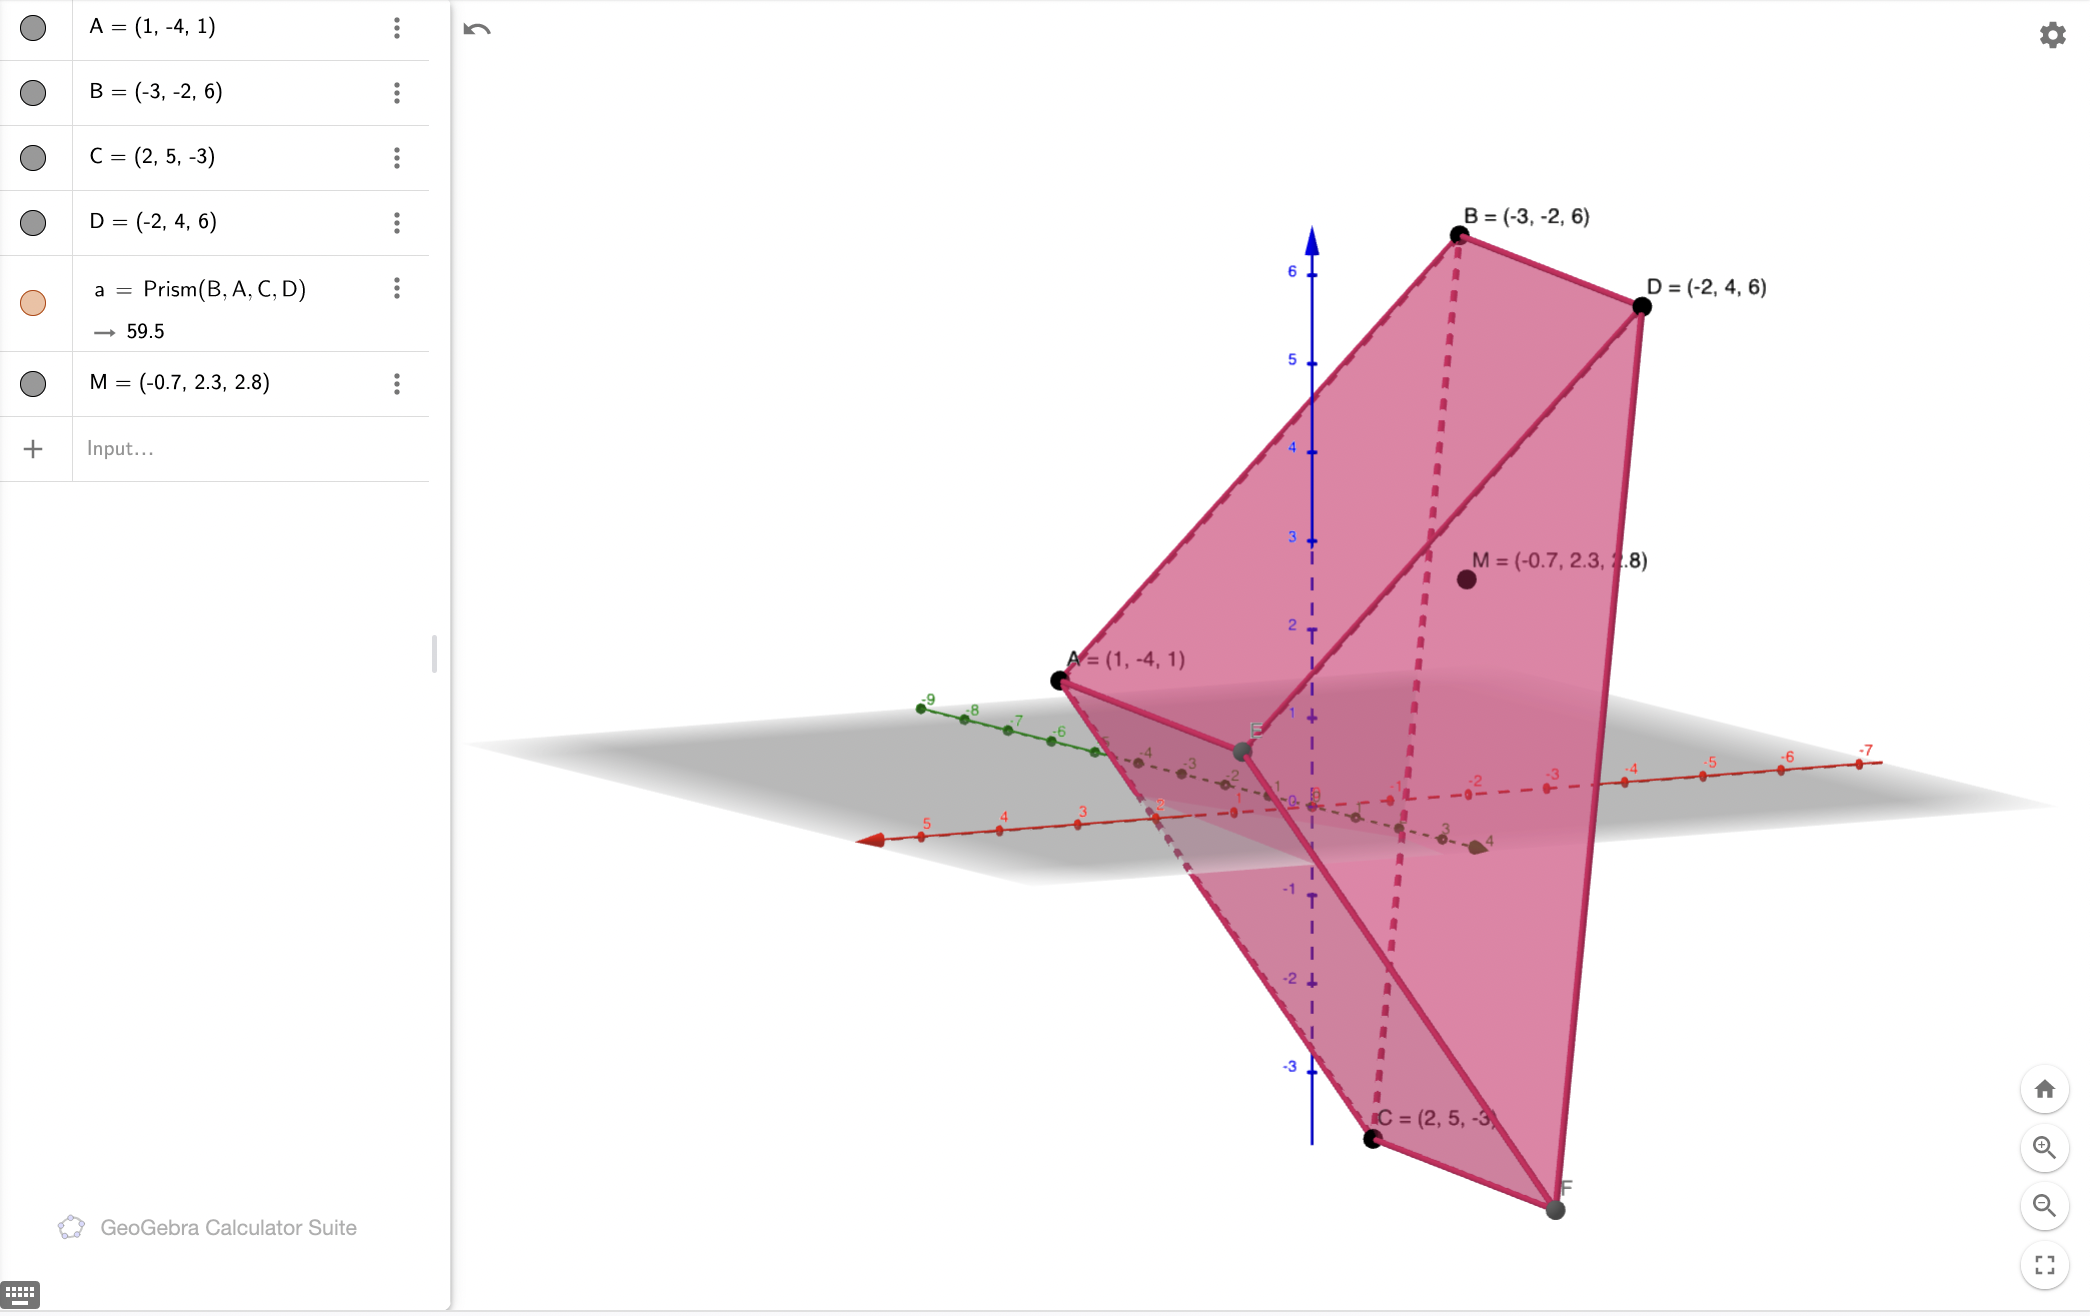
\includegraphics[width=.9\linewidth]{Calculating_the_Center_of_Mass/2021-09-02_21-52-06_screenshot.png}
\end{center}
\end{document}
